\begin{itemize}
\begin{center}
    Paso 24:
\end{center}

    Seguidamente ingresamos al menu principal en modo grafico y hacemos clik en la opcion de Network Connections para poder realizar las configuraciones.
	\begin{center}
	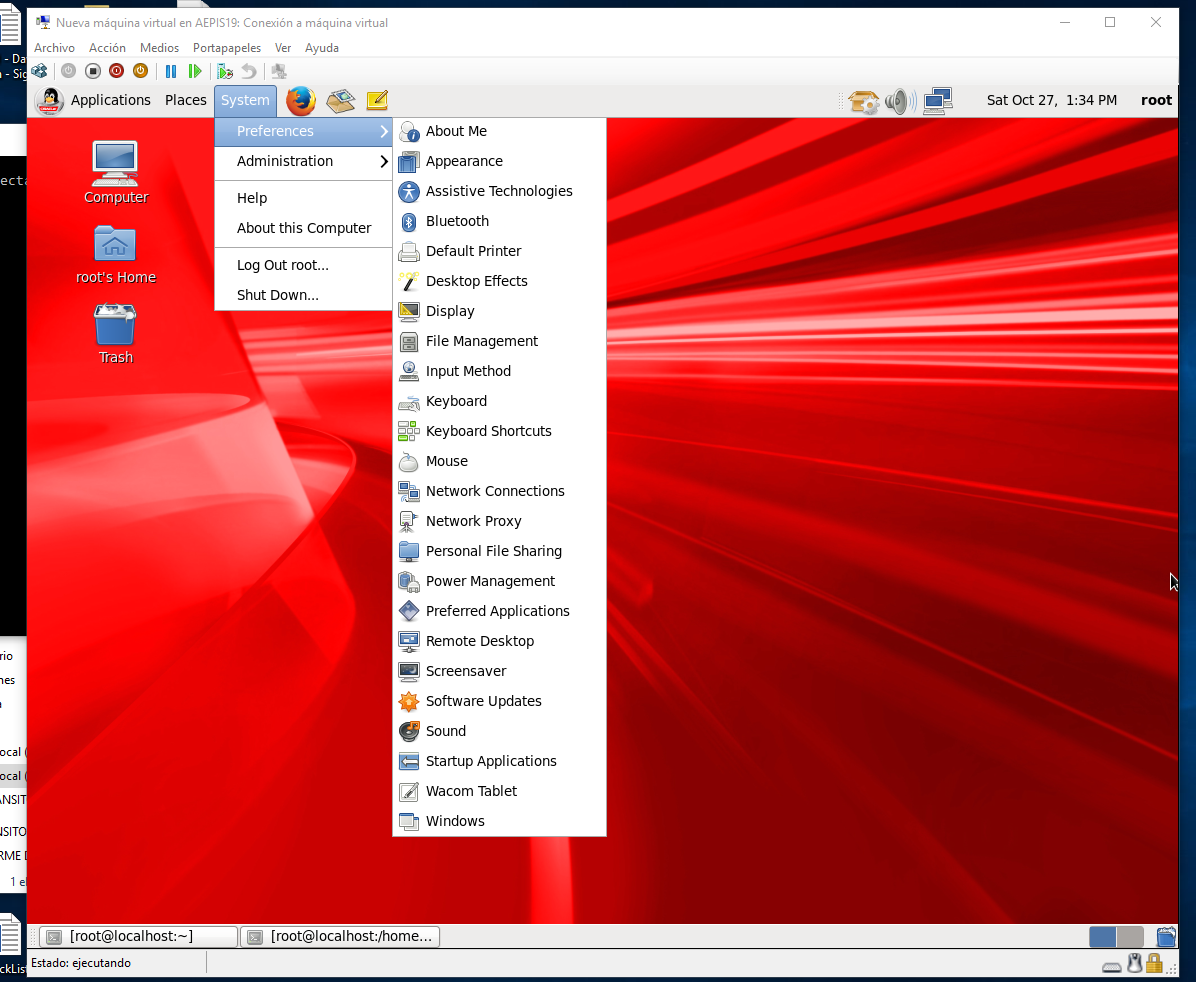
\includegraphics[width=15cm]{./Imagenes/imagen24} 
	\end{center}

\end{itemize} 

\begin{itemize}
\begin{center}
    Paso 25: 
\end{center}

    Luego nos muestra la ventana de de configuracion de IP. 
	\begin{center}
	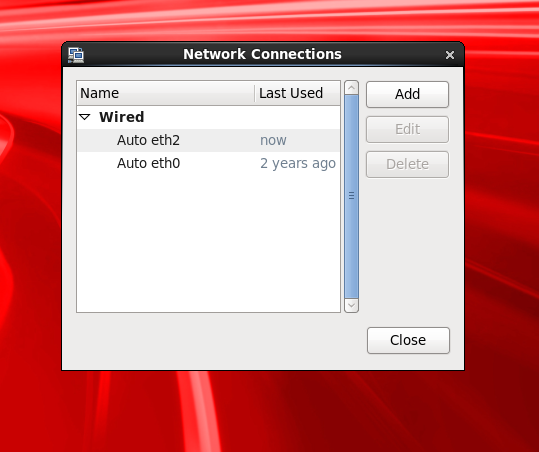
\includegraphics[width=15cm]{./Imagenes/imagen25} 
	\end{center}

\end{itemize} 

\begin{itemize}
\begin{center}
    Paso 26:
\end{center}

    Seguidamente realizamos las asignaciones de IP de forma manual\\
	\begin{center}
	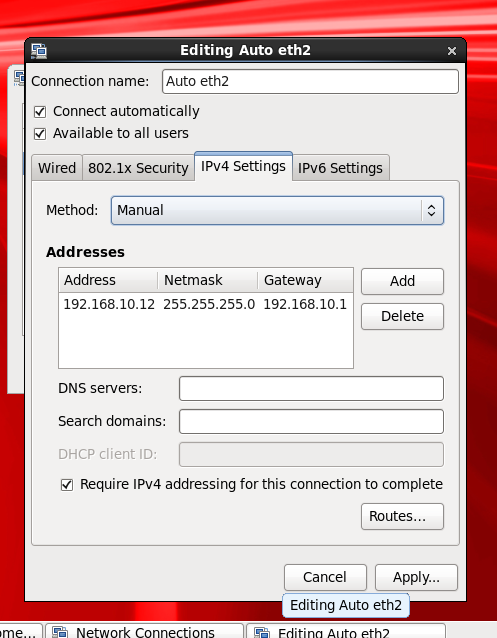
\includegraphics[width=15cm]{./Imagenes/imagen26} 
	\end{center}

\end{itemize} 

\begin{itemize}
\begin{center}
    Paso 27:
\end{center}

    Luego agregamos la configuracion y aceptamos\\
	\begin{center}
	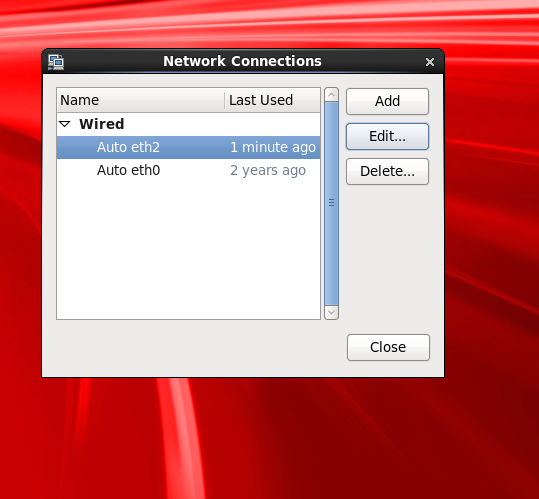
\includegraphics[width=15cm]{./Imagenes/imagen27} 
	\end{center}

\end{itemize} 

\begin{itemize}
\begin{center}
    Paso 28:
\end{center}

    Nos dirigimos a Windows y abrimos el cmd para poder consultar el IP para lo cual utilizamos el ipconfig que nos muestra solo los datos esenciales como la Dirección IP, la Máscara de red y la Puerta de enlace, para cada adaptador encontrado.\\
	\begin{center}
	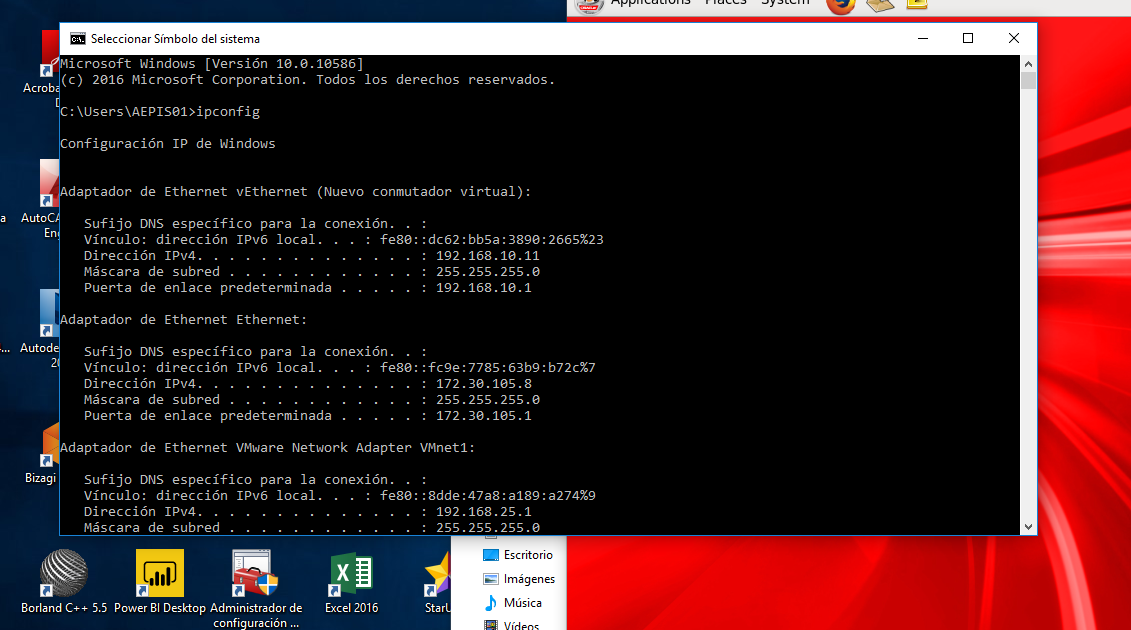
\includegraphics[width=15cm]{./Imagenes/imagen28} 
	\end{center}

\end{itemize} 

\begin{itemize}
\begin{center}
    Paso 29:
\end{center}

    Realizamos el ping que es un comando o una herramienta de diagnóstico que permite hacer una verificación del estado de una determinada conexión de un host local con al menos un equipo remoto contemplado en una red de tipo TCP/IP \\
	\begin{center}
	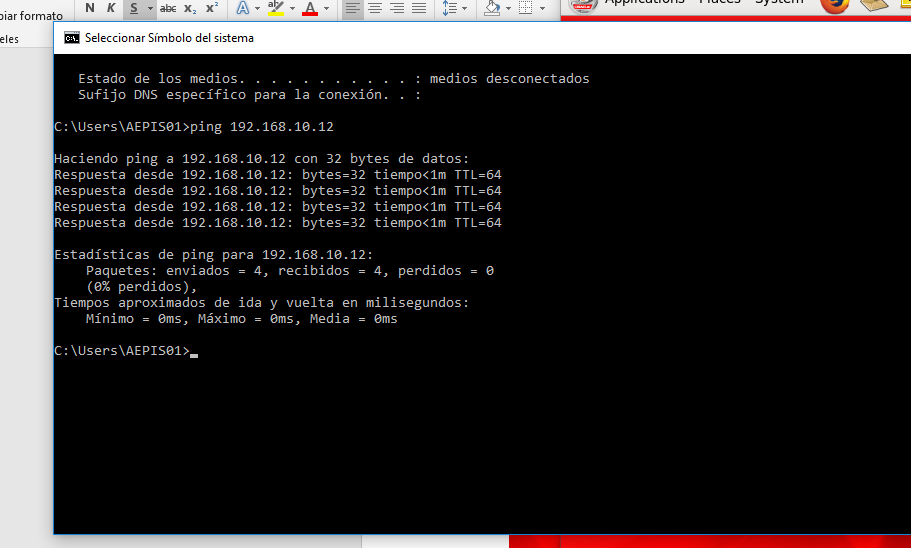
\includegraphics[width=15cm]{./Imagenes/imagen29} 
	\end{center}

\end{itemize} 

\begin{itemize}
\begin{center}
    Paso 30:
\end{center}

    Seguidamente nos dirigimos a nuestra maquina virtual e ingresamos al directorio home \\
	\begin{center}
	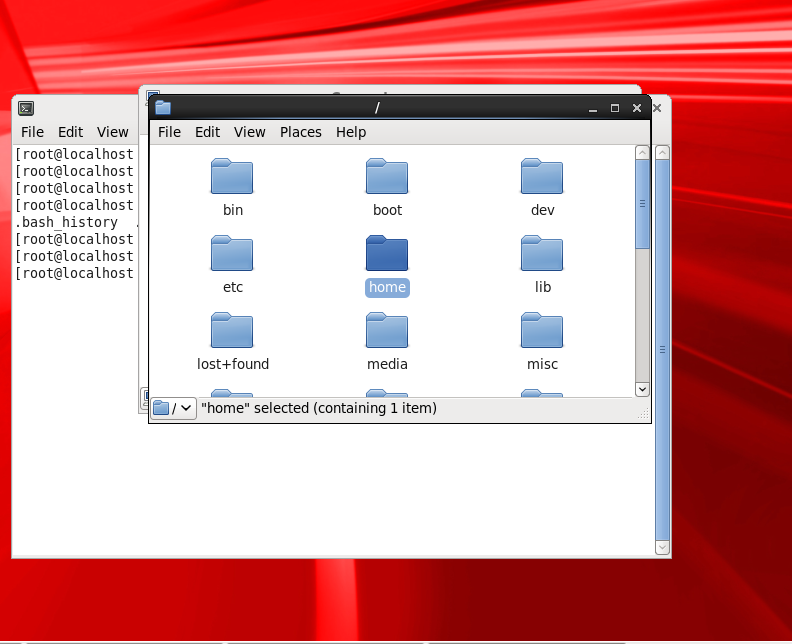
\includegraphics[width=15cm]{./Imagenes/imagen30} 
	\end{center}

\end{itemize} 

\begin{itemize}
\begin{center}
    Paso 31:
\end{center}

    Desconprimimos los 2 archivos que se encuentran\\
	\begin{center}
	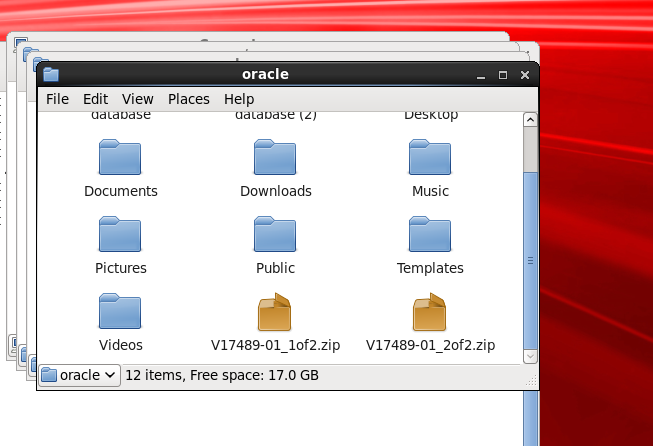
\includegraphics[width=15cm]{./Imagenes/imagen31} 
	\end{center}

\end{itemize} 


\begin{itemize}
\begin{center}
    Paso 32:
\end{center}

    Una vez descomprimido ejecutamos el archivo\\
	\begin{center}
	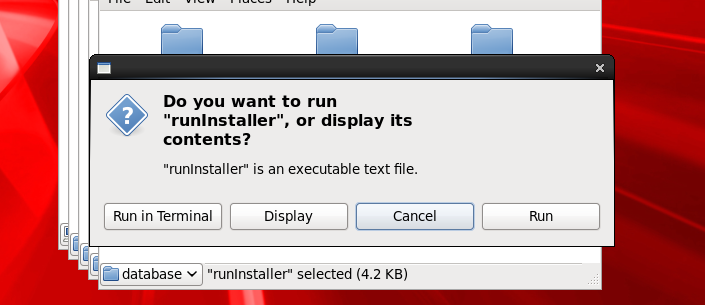
\includegraphics[width=15cm]{./Imagenes/imagen32} 
	\end{center}

\end{itemize} 
